\documentclass[10pt]{article}

\usepackage{amsfonts}
\usepackage{amsmath}
\usepackage{geometry}
\usepackage{amsthm}
\usepackage{mathrsfs}
\usepackage{xcolor,graphicx}
%\usepackage{wrapfig}
\usepackage{subcaption}
%\usepackage{hyperref}

\newgeometry{margin=1in}
\setlength\parindent{0pt}

\DeclareMathOperator{\sgn}{sgn}
\DeclareMathOperator{\Heavi}{H}

\DeclareMathOperator{\Hsign}{\mathscr{H}}
\newcommand\Hank[2][]{{\left( \Hsign_{#1} #2 \right) }}

\newtheorem{theorem}{Theorem}[section]
\newtheorem{definition}[theorem]{Definition}
\newtheorem{corollary}[theorem]{Corollary}

\begin{document}

\section{Analytic Solution}

\subsection{Eigenfunctions of the Laplacian}

\begin{align*}
\nabla^2 \varphi &=0 \\
\varphi &= f(r) g(\theta) h(z) T(t) \\
\nabla^2 &= \frac{1}{r}\frac{\partial}{\partial r} \left( r \frac{\partial}{\partial r} \right) + \frac{1}{r^2} \left( \frac{\partial^2}{\partial \theta^2} \right) + \frac{\partial^2}{\partial z^2} \\
\frac{1}{r}\frac{\partial}{\partial r} \left( r \frac{\partial \varphi}{\partial r} \right) + \frac{1}{r^2} \left( \frac{\partial^2 \varphi}{\partial \theta^2} \right) + \frac{\partial^2 \varphi}{\partial z^2} &= 0 \\
\frac{1}{fr}\frac{\partial}{\partial r}(rf') + \frac{1}{r^2}\frac{g''}{g} + \frac{h''}{h} &= 0 \\
\frac{h''}{h} &= k^2 \\
h(z) &= Ae^{kz} + Be^{-kz} \\
&= e^{kz} \\
\frac{1}{fr}\frac{\partial}{\partial r}(rf') + \frac{1}{r^2}\frac{g''}{g} + k^2 &= 0 \\
\frac{r}{f}\frac{\partial}{\partial r} \left( rf' \right) + k^2r^2 + \frac{g''}{g} &= 0 \\
\frac{g''}{g} &= -\mu^2 \\
g(\theta) &= A \sin(\mu \theta) + B \cos(\mu \theta) \\
\mu &= 0 \\
g(\theta) &= 1 \\
r \frac{\partial}{\partial r}(rf') + (k^2r^2 - 0^2)f &= 0 \\
f(r) &= A J_0(kr) + B Y_0(kr) \\
&= A J_0(kr) \\
\varphi &\propto e^{kz}J_0(kr)T(t) \\
&= \int_0^\infty e^{kz}T(t)J_0(kr)dk
\end{align*}

\subsection{Solving the Velocity Potential}
We must write the gravitational potential as an infinite sum of Bessel functions to match the form of $\varphi$, to do so, we take the Hankel transform,
\begin{align*}
\frac{\partial \Phi}{\partial t}\bigg|_{z=0} &=  \int_0^\infty \Hank{\frac{\partial \Phi}{\partial t}\bigg|_{z=0}}(k) J_0(kr) k \, dk \\
&= G m v^2 t \int_0^\infty \Hank{\frac{1}{(r^2 + v^2 t^2)^{3/2}}}(k) J_0(kr) k \, dk \footnote{hey} \\
&= G m v^2 t \int_0^\infty \frac{1}{|vt|} e^{-k|vt|} J_0(kr) k \, dk \\
&= G m v \sgn(t) \int_0^\infty e^{-kv|t|} J_0(kr) k \, dk.
\end{align*}
\footnotetext{Note that $\int_0^\infty \sqrt{r}(r^2 + v^2 t^2)^{-3/2} dr = \Gamma^2(3/4) (\pi v^3 t^3)^{-1/2} < \infty$ for $t \neq 0$ which is not concerning since this is true almost everywhere, and so the condition in Theorem ***** is satisfied.}
We can now substitute this into the differential equation and find $\varphi$,
\begin{align*}
\int_0^\infty J_0(kr)  \ddot{T}(t) dk + g \int_0^\infty k J_0(kr) T(t) dk + Gmv \int_0^\infty \sgn(t) e^{-kv|t|} J_0(kr)k \, dk = 0 \\
\int_0^\infty \left[ \frac{\ddot{T}(t)}{k} + gT(t) + Gmv \sgn(t) e^{-kv|t|} \right] J_0(kr) k \, dk = 0,
\end{align*}
but, this is nothing more than the Hankel transform of the differential equation for $T$. By taking the Hankel transform of both sides we can remove the integral,
\begin{align*}
\frac{\ddot{T}(t)}{k} + gT(t) + Gmv \sgn(t) e^{-kv|t|} = 0.
\end{align*}
Clearly, the homogeneous solution is $T(t) = A \cos(\omega_k t) + B \sin(\omega_k t)$ with $\omega_k^2 = gk$. The form of the differential equations suggests the form $T(t) = C e^{-kv|t|}$ for the particular solution. Substituting this in yields
\begin{align*}
C \left(k^2 v^2 \sgn^2(t) e^{-kv |t|} + gk e^{-kv |t|} \right) &+ Gmvk \sgn(t) e^{-kv|t|} = 0,
\end{align*}
giving
\begin{align*}
C &= \frac{-Gmvk \sgn(t)}{k^2v^2 + gk} \\
&= \frac{Gmv}{g} \frac{-\sgn(t)}{1+kv^2/g}
\end{align*}
as the coefficient, and,
\begin{align*}
T(t) = \frac{Gmv}{g} \frac{1}{1+kv^2/g} \left( -\sgn(t) e^{-kv|t|} \right) + A \cos(\omega_k t) + B \sin(\omega_k t)
\end{align*}
as the full time component of the velocity potential. We can now apply the boundary conditions to find $A$, and $B$. Physically, we expect $T(t) \in C^1(-\infty,\infty)$, furthermore, we only expect the sinusoidal terms to contribute at times greater than zero, thus,
\begin{align*}
T(t) &= \frac{Gmv}{g}\frac{1}{1+kv^2/g} \left(-\sgn(t)e^{-kv|t|} + 2H(t)\cos(\omega_k t) \right)dk, \text{ and,} \\
\varphi &= \frac{Gmv}{g} \int_0^\infty \frac{J_0(kr)e^{kz}}{1+kv^2/g} \left(-\sgn(t)e^{-kv|t|} + 2H(t)\cos(\omega_k t) \right)dk.
\end{align*}

\begin{align*}
\varphi = \int_0^\infty J_0(kr) e^{kz} T(t) dk \\
\left( \frac{\partial \varphi}{\partial t} + (g \eta + \Phi) \right) \bigg|_{z=0} = 0 \\
\left( \frac{\partial^2 \varphi}{\partial t^2} + g \frac{\partial \varphi}{\partial z} + \frac{\partial \Phi}{\partial t} \right) \bigg|_{z=0} = 0\\
\text{where }\Phi = \frac{-Gm}{\sqrt{r^2+(z-vt)^2}} \\
\varphi = \frac{Gmv}{g} \int_0^\infty \frac{J_0(kr)e^{kz}}{1+kv^2/g} \left(-\sgn(t)e^{-kv|t|} + 2 \Heavi (t)\cos(\omega_k t) \right)dk \\
\text{with } \omega_k^2=gk
\end{align*}

\newpage

\begin{figure}[p]
\begin{centering}
 \begin{subfigure}{\textwidth}
  % GNUPLOT: LaTeX picture with Postscript
\begingroup
  \makeatletter
  \providecommand\color[2][]{%
    \GenericError{(gnuplot) \space\space\space\@spaces}{%
      Package color not loaded in conjunction with
      terminal option `colourtext'%
    }{See the gnuplot documentation for explanation.%
    }{Either use 'blacktext' in gnuplot or load the package
      color.sty in LaTeX.}%
    \renewcommand\color[2][]{}%
  }%
  \providecommand\includegraphics[2][]{%
    \GenericError{(gnuplot) \space\space\space\@spaces}{%
      Package graphicx or graphics not loaded%
    }{See the gnuplot documentation for explanation.%
    }{The gnuplot epslatex terminal needs graphicx.sty or graphics.sty.}%
    \renewcommand\includegraphics[2][]{}%
  }%
  \providecommand\rotatebox[2]{#2}%
  \@ifundefined{ifGPcolor}{%
    \newif\ifGPcolor
    \GPcolortrue
  }{}%
  \@ifundefined{ifGPblacktext}{%
    \newif\ifGPblacktext
    \GPblacktexttrue
  }{}%
  % define a \g@addto@macro without @ in the name:
  \let\gplgaddtomacro\g@addto@macro
  % define empty templates for all commands taking text:
  \gdef\gplbacktext{}%
  \gdef\gplfronttext{}%
  \makeatother
  \ifGPblacktext
    % no textcolor at all
    \def\colorrgb#1{}%
    \def\colorgray#1{}%
  \else
    % gray or color?
    \ifGPcolor
      \def\colorrgb#1{\color[rgb]{#1}}%
      \def\colorgray#1{\color[gray]{#1}}%
      \expandafter\def\csname LTw\endcsname{\color{white}}%
      \expandafter\def\csname LTb\endcsname{\color{black}}%
      \expandafter\def\csname LTa\endcsname{\color{black}}%
      \expandafter\def\csname LT0\endcsname{\color[rgb]{1,0,0}}%
      \expandafter\def\csname LT1\endcsname{\color[rgb]{0,1,0}}%
      \expandafter\def\csname LT2\endcsname{\color[rgb]{0,0,1}}%
      \expandafter\def\csname LT3\endcsname{\color[rgb]{1,0,1}}%
      \expandafter\def\csname LT4\endcsname{\color[rgb]{0,1,1}}%
      \expandafter\def\csname LT5\endcsname{\color[rgb]{1,1,0}}%
      \expandafter\def\csname LT6\endcsname{\color[rgb]{0,0,0}}%
      \expandafter\def\csname LT7\endcsname{\color[rgb]{1,0.3,0}}%
      \expandafter\def\csname LT8\endcsname{\color[rgb]{0.5,0.5,0.5}}%
    \else
      % gray
      \def\colorrgb#1{\color{black}}%
      \def\colorgray#1{\color[gray]{#1}}%
      \expandafter\def\csname LTw\endcsname{\color{white}}%
      \expandafter\def\csname LTb\endcsname{\color{black}}%
      \expandafter\def\csname LTa\endcsname{\color{black}}%
      \expandafter\def\csname LT0\endcsname{\color{black}}%
      \expandafter\def\csname LT1\endcsname{\color{black}}%
      \expandafter\def\csname LT2\endcsname{\color{black}}%
      \expandafter\def\csname LT3\endcsname{\color{black}}%
      \expandafter\def\csname LT4\endcsname{\color{black}}%
      \expandafter\def\csname LT5\endcsname{\color{black}}%
      \expandafter\def\csname LT6\endcsname{\color{black}}%
      \expandafter\def\csname LT7\endcsname{\color{black}}%
      \expandafter\def\csname LT8\endcsname{\color{black}}%
    \fi
  \fi
    \setlength{\unitlength}{0.0500bp}%
    \ifx\gptboxheight\undefined%
      \newlength{\gptboxheight}%
      \newlength{\gptboxwidth}%
      \newsavebox{\gptboxtext}%
    \fi%
    \setlength{\fboxrule}{0.5pt}%
    \setlength{\fboxsep}{1pt}%
\begin{picture}(8640.00,3600.00)%
    \gplgaddtomacro\gplbacktext{%
    }%
    \gplgaddtomacro\gplfronttext{%
      \csname LTb\endcsname%
      \put(176,2019){\makebox(0,0){\strut{}$\eta \cdot \frac{v^2}{Gm}$}}%
      \put(4528,154){\makebox(0,0){\strut{}$r \cdot \frac{g}{v^2}$}}%
      \csname LTb\endcsname%
      \put(682,704){\makebox(0,0)[r]{\strut{}$-4$}}%
      \csname LTb\endcsname%
      \put(682,1581){\makebox(0,0)[r]{\strut{}$0$}}%
      \csname LTb\endcsname%
      \put(682,2458){\makebox(0,0)[r]{\strut{}$4$}}%
      \csname LTb\endcsname%
      \put(682,3335){\makebox(0,0)[r]{\strut{}$8$}}%
      \csname LTb\endcsname%
      \put(1987,484){\makebox(0,0){\strut{}$0.2$}}%
      \csname LTb\endcsname%
      \put(3551,484){\makebox(0,0){\strut{}$0.4$}}%
      \csname LTb\endcsname%
      \put(5115,484){\makebox(0,0){\strut{}$0.6$}}%
      \csname LTb\endcsname%
      \put(6679,484){\makebox(0,0){\strut{}$0.8$}}%
      \csname LTb\endcsname%
      \put(8243,484){\makebox(0,0){\strut{}$1$}}%
    }%
    \gplbacktext
    \put(0,0){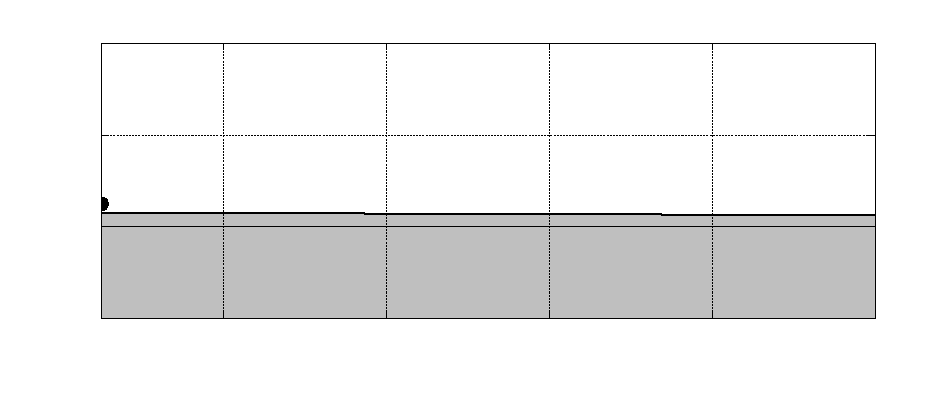
\includegraphics{./Analytic000}}%
    \gplfronttext
  \end{picture}%
\endgroup

  \caption{$t=-1$ s.}
 \end{subfigure} \\
 \begin{subfigure}{\textwidth}
  % GNUPLOT: LaTeX picture with Postscript
\begingroup
  \makeatletter
  \providecommand\color[2][]{%
    \GenericError{(gnuplot) \space\space\space\@spaces}{%
      Package color not loaded in conjunction with
      terminal option `colourtext'%
    }{See the gnuplot documentation for explanation.%
    }{Either use 'blacktext' in gnuplot or load the package
      color.sty in LaTeX.}%
    \renewcommand\color[2][]{}%
  }%
  \providecommand\includegraphics[2][]{%
    \GenericError{(gnuplot) \space\space\space\@spaces}{%
      Package graphicx or graphics not loaded%
    }{See the gnuplot documentation for explanation.%
    }{The gnuplot epslatex terminal needs graphicx.sty or graphics.sty.}%
    \renewcommand\includegraphics[2][]{}%
  }%
  \providecommand\rotatebox[2]{#2}%
  \@ifundefined{ifGPcolor}{%
    \newif\ifGPcolor
    \GPcolortrue
  }{}%
  \@ifundefined{ifGPblacktext}{%
    \newif\ifGPblacktext
    \GPblacktexttrue
  }{}%
  % define a \g@addto@macro without @ in the name:
  \let\gplgaddtomacro\g@addto@macro
  % define empty templates for all commands taking text:
  \gdef\gplbacktext{}%
  \gdef\gplfronttext{}%
  \makeatother
  \ifGPblacktext
    % no textcolor at all
    \def\colorrgb#1{}%
    \def\colorgray#1{}%
  \else
    % gray or color?
    \ifGPcolor
      \def\colorrgb#1{\color[rgb]{#1}}%
      \def\colorgray#1{\color[gray]{#1}}%
      \expandafter\def\csname LTw\endcsname{\color{white}}%
      \expandafter\def\csname LTb\endcsname{\color{black}}%
      \expandafter\def\csname LTa\endcsname{\color{black}}%
      \expandafter\def\csname LT0\endcsname{\color[rgb]{1,0,0}}%
      \expandafter\def\csname LT1\endcsname{\color[rgb]{0,1,0}}%
      \expandafter\def\csname LT2\endcsname{\color[rgb]{0,0,1}}%
      \expandafter\def\csname LT3\endcsname{\color[rgb]{1,0,1}}%
      \expandafter\def\csname LT4\endcsname{\color[rgb]{0,1,1}}%
      \expandafter\def\csname LT5\endcsname{\color[rgb]{1,1,0}}%
      \expandafter\def\csname LT6\endcsname{\color[rgb]{0,0,0}}%
      \expandafter\def\csname LT7\endcsname{\color[rgb]{1,0.3,0}}%
      \expandafter\def\csname LT8\endcsname{\color[rgb]{0.5,0.5,0.5}}%
    \else
      % gray
      \def\colorrgb#1{\color{black}}%
      \def\colorgray#1{\color[gray]{#1}}%
      \expandafter\def\csname LTw\endcsname{\color{white}}%
      \expandafter\def\csname LTb\endcsname{\color{black}}%
      \expandafter\def\csname LTa\endcsname{\color{black}}%
      \expandafter\def\csname LT0\endcsname{\color{black}}%
      \expandafter\def\csname LT1\endcsname{\color{black}}%
      \expandafter\def\csname LT2\endcsname{\color{black}}%
      \expandafter\def\csname LT3\endcsname{\color{black}}%
      \expandafter\def\csname LT4\endcsname{\color{black}}%
      \expandafter\def\csname LT5\endcsname{\color{black}}%
      \expandafter\def\csname LT6\endcsname{\color{black}}%
      \expandafter\def\csname LT7\endcsname{\color{black}}%
      \expandafter\def\csname LT8\endcsname{\color{black}}%
    \fi
  \fi
    \setlength{\unitlength}{0.0500bp}%
    \ifx\gptboxheight\undefined%
      \newlength{\gptboxheight}%
      \newlength{\gptboxwidth}%
      \newsavebox{\gptboxtext}%
    \fi%
    \setlength{\fboxrule}{0.5pt}%
    \setlength{\fboxsep}{1pt}%
\begin{picture}(8640.00,3600.00)%
    \gplgaddtomacro\gplbacktext{%
    }%
    \gplgaddtomacro\gplfronttext{%
      \csname LTb\endcsname%
      \put(176,2019){\makebox(0,0){\strut{}$\eta \cdot \frac{v^2}{Gm}$}}%
      \put(4528,154){\makebox(0,0){\strut{}$r \cdot \frac{g}{v^2}$}}%
      \csname LTb\endcsname%
      \put(682,704){\makebox(0,0)[r]{\strut{}$-4$}}%
      \csname LTb\endcsname%
      \put(682,1581){\makebox(0,0)[r]{\strut{}$0$}}%
      \csname LTb\endcsname%
      \put(682,2458){\makebox(0,0)[r]{\strut{}$4$}}%
      \csname LTb\endcsname%
      \put(682,3335){\makebox(0,0)[r]{\strut{}$8$}}%
      \csname LTb\endcsname%
      \put(1987,484){\makebox(0,0){\strut{}$0.2$}}%
      \csname LTb\endcsname%
      \put(3551,484){\makebox(0,0){\strut{}$0.4$}}%
      \csname LTb\endcsname%
      \put(5115,484){\makebox(0,0){\strut{}$0.6$}}%
      \csname LTb\endcsname%
      \put(6679,484){\makebox(0,0){\strut{}$0.8$}}%
      \csname LTb\endcsname%
      \put(8243,484){\makebox(0,0){\strut{}$1$}}%
    }%
    \gplbacktext
    \put(0,0){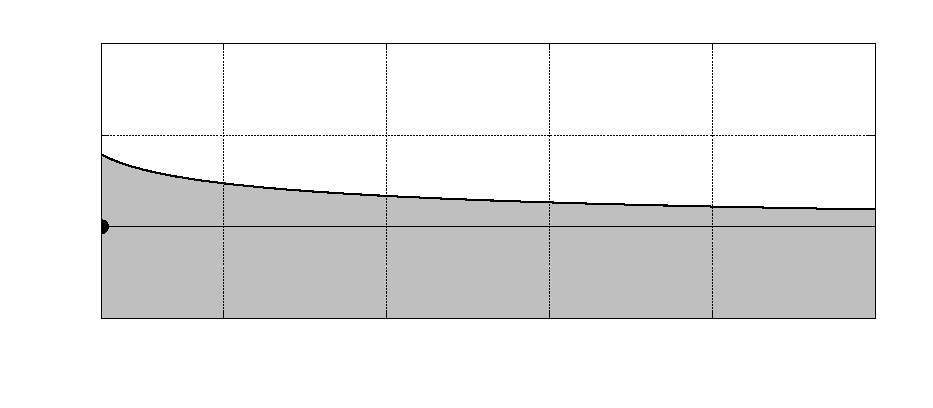
\includegraphics{./Analytic001}}%
    \gplfronttext
  \end{picture}%
\endgroup

  \caption{$t=0$ s.}
 \end{subfigure} \\
 \begin{subfigure}{\textwidth}
  % GNUPLOT: LaTeX picture with Postscript
\begingroup
  \makeatletter
  \providecommand\color[2][]{%
    \GenericError{(gnuplot) \space\space\space\@spaces}{%
      Package color not loaded in conjunction with
      terminal option `colourtext'%
    }{See the gnuplot documentation for explanation.%
    }{Either use 'blacktext' in gnuplot or load the package
      color.sty in LaTeX.}%
    \renewcommand\color[2][]{}%
  }%
  \providecommand\includegraphics[2][]{%
    \GenericError{(gnuplot) \space\space\space\@spaces}{%
      Package graphicx or graphics not loaded%
    }{See the gnuplot documentation for explanation.%
    }{The gnuplot epslatex terminal needs graphicx.sty or graphics.sty.}%
    \renewcommand\includegraphics[2][]{}%
  }%
  \providecommand\rotatebox[2]{#2}%
  \@ifundefined{ifGPcolor}{%
    \newif\ifGPcolor
    \GPcolortrue
  }{}%
  \@ifundefined{ifGPblacktext}{%
    \newif\ifGPblacktext
    \GPblacktexttrue
  }{}%
  % define a \g@addto@macro without @ in the name:
  \let\gplgaddtomacro\g@addto@macro
  % define empty templates for all commands taking text:
  \gdef\gplbacktext{}%
  \gdef\gplfronttext{}%
  \makeatother
  \ifGPblacktext
    % no textcolor at all
    \def\colorrgb#1{}%
    \def\colorgray#1{}%
  \else
    % gray or color?
    \ifGPcolor
      \def\colorrgb#1{\color[rgb]{#1}}%
      \def\colorgray#1{\color[gray]{#1}}%
      \expandafter\def\csname LTw\endcsname{\color{white}}%
      \expandafter\def\csname LTb\endcsname{\color{black}}%
      \expandafter\def\csname LTa\endcsname{\color{black}}%
      \expandafter\def\csname LT0\endcsname{\color[rgb]{1,0,0}}%
      \expandafter\def\csname LT1\endcsname{\color[rgb]{0,1,0}}%
      \expandafter\def\csname LT2\endcsname{\color[rgb]{0,0,1}}%
      \expandafter\def\csname LT3\endcsname{\color[rgb]{1,0,1}}%
      \expandafter\def\csname LT4\endcsname{\color[rgb]{0,1,1}}%
      \expandafter\def\csname LT5\endcsname{\color[rgb]{1,1,0}}%
      \expandafter\def\csname LT6\endcsname{\color[rgb]{0,0,0}}%
      \expandafter\def\csname LT7\endcsname{\color[rgb]{1,0.3,0}}%
      \expandafter\def\csname LT8\endcsname{\color[rgb]{0.5,0.5,0.5}}%
    \else
      % gray
      \def\colorrgb#1{\color{black}}%
      \def\colorgray#1{\color[gray]{#1}}%
      \expandafter\def\csname LTw\endcsname{\color{white}}%
      \expandafter\def\csname LTb\endcsname{\color{black}}%
      \expandafter\def\csname LTa\endcsname{\color{black}}%
      \expandafter\def\csname LT0\endcsname{\color{black}}%
      \expandafter\def\csname LT1\endcsname{\color{black}}%
      \expandafter\def\csname LT2\endcsname{\color{black}}%
      \expandafter\def\csname LT3\endcsname{\color{black}}%
      \expandafter\def\csname LT4\endcsname{\color{black}}%
      \expandafter\def\csname LT5\endcsname{\color{black}}%
      \expandafter\def\csname LT6\endcsname{\color{black}}%
      \expandafter\def\csname LT7\endcsname{\color{black}}%
      \expandafter\def\csname LT8\endcsname{\color{black}}%
    \fi
  \fi
    \setlength{\unitlength}{0.0500bp}%
    \ifx\gptboxheight\undefined%
      \newlength{\gptboxheight}%
      \newlength{\gptboxwidth}%
      \newsavebox{\gptboxtext}%
    \fi%
    \setlength{\fboxrule}{0.5pt}%
    \setlength{\fboxsep}{1pt}%
\begin{picture}(8640.00,3600.00)%
    \gplgaddtomacro\gplbacktext{%
    }%
    \gplgaddtomacro\gplfronttext{%
      \csname LTb\endcsname%
      \put(176,2019){\makebox(0,0){\strut{}$\eta \cdot \frac{v^2}{Gm}$}}%
      \put(4528,154){\makebox(0,0){\strut{}$r \cdot \frac{g}{v^2}$}}%
      \csname LTb\endcsname%
      \put(682,704){\makebox(0,0)[r]{\strut{}$-4$}}%
      \csname LTb\endcsname%
      \put(682,1581){\makebox(0,0)[r]{\strut{}$0$}}%
      \csname LTb\endcsname%
      \put(682,2458){\makebox(0,0)[r]{\strut{}$4$}}%
      \csname LTb\endcsname%
      \put(682,3335){\makebox(0,0)[r]{\strut{}$8$}}%
      \csname LTb\endcsname%
      \put(1987,484){\makebox(0,0){\strut{}$0.2$}}%
      \csname LTb\endcsname%
      \put(3551,484){\makebox(0,0){\strut{}$0.4$}}%
      \csname LTb\endcsname%
      \put(5115,484){\makebox(0,0){\strut{}$0.6$}}%
      \csname LTb\endcsname%
      \put(6679,484){\makebox(0,0){\strut{}$0.8$}}%
      \csname LTb\endcsname%
      \put(8243,484){\makebox(0,0){\strut{}$1$}}%
    }%
    \gplbacktext
    \put(0,0){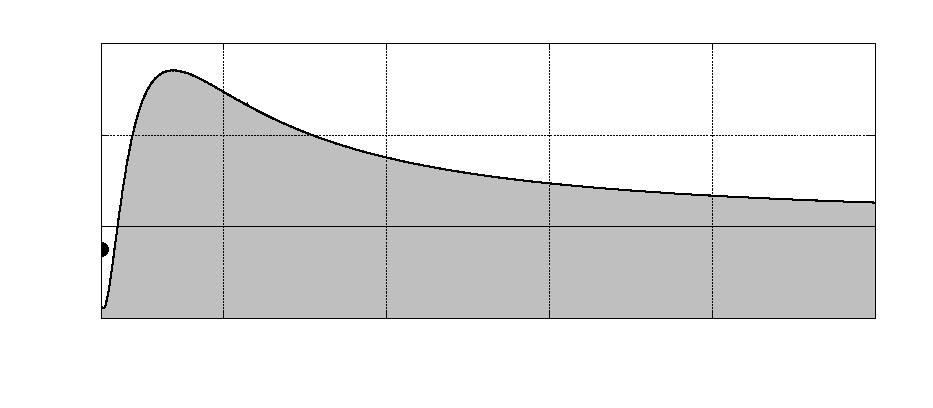
\includegraphics{./Analytic002}}%
    \gplfronttext
  \end{picture}%
\endgroup

  \caption{$t=1$ s.}
 \end{subfigure}
\end{centering}
\end{figure}

\begin{figure}[p] \ContinuedFloat
\begin{centering}
 \begin{subfigure}{\textwidth}
  % GNUPLOT: LaTeX picture with Postscript
\begingroup
  \makeatletter
  \providecommand\color[2][]{%
    \GenericError{(gnuplot) \space\space\space\@spaces}{%
      Package color not loaded in conjunction with
      terminal option `colourtext'%
    }{See the gnuplot documentation for explanation.%
    }{Either use 'blacktext' in gnuplot or load the package
      color.sty in LaTeX.}%
    \renewcommand\color[2][]{}%
  }%
  \providecommand\includegraphics[2][]{%
    \GenericError{(gnuplot) \space\space\space\@spaces}{%
      Package graphicx or graphics not loaded%
    }{See the gnuplot documentation for explanation.%
    }{The gnuplot epslatex terminal needs graphicx.sty or graphics.sty.}%
    \renewcommand\includegraphics[2][]{}%
  }%
  \providecommand\rotatebox[2]{#2}%
  \@ifundefined{ifGPcolor}{%
    \newif\ifGPcolor
    \GPcolortrue
  }{}%
  \@ifundefined{ifGPblacktext}{%
    \newif\ifGPblacktext
    \GPblacktexttrue
  }{}%
  % define a \g@addto@macro without @ in the name:
  \let\gplgaddtomacro\g@addto@macro
  % define empty templates for all commands taking text:
  \gdef\gplbacktext{}%
  \gdef\gplfronttext{}%
  \makeatother
  \ifGPblacktext
    % no textcolor at all
    \def\colorrgb#1{}%
    \def\colorgray#1{}%
  \else
    % gray or color?
    \ifGPcolor
      \def\colorrgb#1{\color[rgb]{#1}}%
      \def\colorgray#1{\color[gray]{#1}}%
      \expandafter\def\csname LTw\endcsname{\color{white}}%
      \expandafter\def\csname LTb\endcsname{\color{black}}%
      \expandafter\def\csname LTa\endcsname{\color{black}}%
      \expandafter\def\csname LT0\endcsname{\color[rgb]{1,0,0}}%
      \expandafter\def\csname LT1\endcsname{\color[rgb]{0,1,0}}%
      \expandafter\def\csname LT2\endcsname{\color[rgb]{0,0,1}}%
      \expandafter\def\csname LT3\endcsname{\color[rgb]{1,0,1}}%
      \expandafter\def\csname LT4\endcsname{\color[rgb]{0,1,1}}%
      \expandafter\def\csname LT5\endcsname{\color[rgb]{1,1,0}}%
      \expandafter\def\csname LT6\endcsname{\color[rgb]{0,0,0}}%
      \expandafter\def\csname LT7\endcsname{\color[rgb]{1,0.3,0}}%
      \expandafter\def\csname LT8\endcsname{\color[rgb]{0.5,0.5,0.5}}%
    \else
      % gray
      \def\colorrgb#1{\color{black}}%
      \def\colorgray#1{\color[gray]{#1}}%
      \expandafter\def\csname LTw\endcsname{\color{white}}%
      \expandafter\def\csname LTb\endcsname{\color{black}}%
      \expandafter\def\csname LTa\endcsname{\color{black}}%
      \expandafter\def\csname LT0\endcsname{\color{black}}%
      \expandafter\def\csname LT1\endcsname{\color{black}}%
      \expandafter\def\csname LT2\endcsname{\color{black}}%
      \expandafter\def\csname LT3\endcsname{\color{black}}%
      \expandafter\def\csname LT4\endcsname{\color{black}}%
      \expandafter\def\csname LT5\endcsname{\color{black}}%
      \expandafter\def\csname LT6\endcsname{\color{black}}%
      \expandafter\def\csname LT7\endcsname{\color{black}}%
      \expandafter\def\csname LT8\endcsname{\color{black}}%
    \fi
  \fi
    \setlength{\unitlength}{0.0500bp}%
    \ifx\gptboxheight\undefined%
      \newlength{\gptboxheight}%
      \newlength{\gptboxwidth}%
      \newsavebox{\gptboxtext}%
    \fi%
    \setlength{\fboxrule}{0.5pt}%
    \setlength{\fboxsep}{1pt}%
\begin{picture}(8640.00,3600.00)%
    \gplgaddtomacro\gplbacktext{%
    }%
    \gplgaddtomacro\gplfronttext{%
      \csname LTb\endcsname%
      \put(176,2019){\makebox(0,0){\strut{}$\frac{\eta}{Gm/v^2}$}}%
      \put(4528,154){\makebox(0,0){\strut{}$\chi$}}%
      \csname LTb\endcsname%
      \put(682,704){\makebox(0,0)[r]{\strut{}$-4$}}%
      \csname LTb\endcsname%
      \put(682,1581){\makebox(0,0)[r]{\strut{}$0$}}%
      \csname LTb\endcsname%
      \put(682,2458){\makebox(0,0)[r]{\strut{}$4$}}%
      \csname LTb\endcsname%
      \put(682,3335){\makebox(0,0)[r]{\strut{}$8$}}%
      \csname LTb\endcsname%
      \put(1987,484){\makebox(0,0){\strut{}$0.2$}}%
      \csname LTb\endcsname%
      \put(3551,484){\makebox(0,0){\strut{}$0.4$}}%
      \csname LTb\endcsname%
      \put(5115,484){\makebox(0,0){\strut{}$0.6$}}%
      \csname LTb\endcsname%
      \put(6679,484){\makebox(0,0){\strut{}$0.8$}}%
      \csname LTb\endcsname%
      \put(8243,484){\makebox(0,0){\strut{}$1$}}%
    }%
    \gplbacktext
    \put(0,0){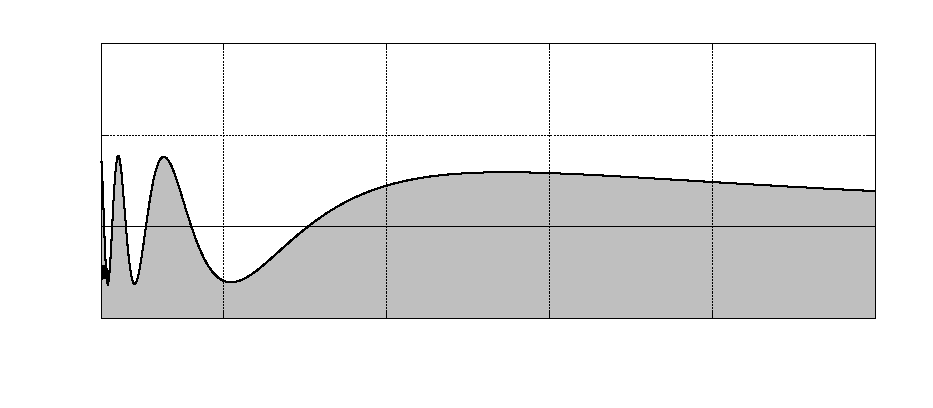
\includegraphics{./3Analytic/Analytic003}}%
    \gplfronttext
  \end{picture}%
\endgroup

  \caption{$t=2$ s.}
 \end{subfigure} \\
 \begin{subfigure}{\textwidth}
  % GNUPLOT: LaTeX picture with Postscript
\begingroup
  \makeatletter
  \providecommand\color[2][]{%
    \GenericError{(gnuplot) \space\space\space\@spaces}{%
      Package color not loaded in conjunction with
      terminal option `colourtext'%
    }{See the gnuplot documentation for explanation.%
    }{Either use 'blacktext' in gnuplot or load the package
      color.sty in LaTeX.}%
    \renewcommand\color[2][]{}%
  }%
  \providecommand\includegraphics[2][]{%
    \GenericError{(gnuplot) \space\space\space\@spaces}{%
      Package graphicx or graphics not loaded%
    }{See the gnuplot documentation for explanation.%
    }{The gnuplot epslatex terminal needs graphicx.sty or graphics.sty.}%
    \renewcommand\includegraphics[2][]{}%
  }%
  \providecommand\rotatebox[2]{#2}%
  \@ifundefined{ifGPcolor}{%
    \newif\ifGPcolor
    \GPcolortrue
  }{}%
  \@ifundefined{ifGPblacktext}{%
    \newif\ifGPblacktext
    \GPblacktexttrue
  }{}%
  % define a \g@addto@macro without @ in the name:
  \let\gplgaddtomacro\g@addto@macro
  % define empty templates for all commands taking text:
  \gdef\gplbacktext{}%
  \gdef\gplfronttext{}%
  \makeatother
  \ifGPblacktext
    % no textcolor at all
    \def\colorrgb#1{}%
    \def\colorgray#1{}%
  \else
    % gray or color?
    \ifGPcolor
      \def\colorrgb#1{\color[rgb]{#1}}%
      \def\colorgray#1{\color[gray]{#1}}%
      \expandafter\def\csname LTw\endcsname{\color{white}}%
      \expandafter\def\csname LTb\endcsname{\color{black}}%
      \expandafter\def\csname LTa\endcsname{\color{black}}%
      \expandafter\def\csname LT0\endcsname{\color[rgb]{1,0,0}}%
      \expandafter\def\csname LT1\endcsname{\color[rgb]{0,1,0}}%
      \expandafter\def\csname LT2\endcsname{\color[rgb]{0,0,1}}%
      \expandafter\def\csname LT3\endcsname{\color[rgb]{1,0,1}}%
      \expandafter\def\csname LT4\endcsname{\color[rgb]{0,1,1}}%
      \expandafter\def\csname LT5\endcsname{\color[rgb]{1,1,0}}%
      \expandafter\def\csname LT6\endcsname{\color[rgb]{0,0,0}}%
      \expandafter\def\csname LT7\endcsname{\color[rgb]{1,0.3,0}}%
      \expandafter\def\csname LT8\endcsname{\color[rgb]{0.5,0.5,0.5}}%
    \else
      % gray
      \def\colorrgb#1{\color{black}}%
      \def\colorgray#1{\color[gray]{#1}}%
      \expandafter\def\csname LTw\endcsname{\color{white}}%
      \expandafter\def\csname LTb\endcsname{\color{black}}%
      \expandafter\def\csname LTa\endcsname{\color{black}}%
      \expandafter\def\csname LT0\endcsname{\color{black}}%
      \expandafter\def\csname LT1\endcsname{\color{black}}%
      \expandafter\def\csname LT2\endcsname{\color{black}}%
      \expandafter\def\csname LT3\endcsname{\color{black}}%
      \expandafter\def\csname LT4\endcsname{\color{black}}%
      \expandafter\def\csname LT5\endcsname{\color{black}}%
      \expandafter\def\csname LT6\endcsname{\color{black}}%
      \expandafter\def\csname LT7\endcsname{\color{black}}%
      \expandafter\def\csname LT8\endcsname{\color{black}}%
    \fi
  \fi
    \setlength{\unitlength}{0.0500bp}%
    \ifx\gptboxheight\undefined%
      \newlength{\gptboxheight}%
      \newlength{\gptboxwidth}%
      \newsavebox{\gptboxtext}%
    \fi%
    \setlength{\fboxrule}{0.5pt}%
    \setlength{\fboxsep}{1pt}%
\begin{picture}(8640.00,3600.00)%
    \gplgaddtomacro\gplbacktext{%
    }%
    \gplgaddtomacro\gplfronttext{%
      \csname LTb\endcsname%
      \put(176,2019){\makebox(0,0){\strut{}$\eta \cdot \frac{v^2}{Gm}$}}%
      \put(4528,154){\makebox(0,0){\strut{}$r \cdot \frac{g}{v^2}$}}%
      \csname LTb\endcsname%
      \put(682,704){\makebox(0,0)[r]{\strut{}$-4$}}%
      \csname LTb\endcsname%
      \put(682,1581){\makebox(0,0)[r]{\strut{}$0$}}%
      \csname LTb\endcsname%
      \put(682,2458){\makebox(0,0)[r]{\strut{}$4$}}%
      \csname LTb\endcsname%
      \put(682,3335){\makebox(0,0)[r]{\strut{}$8$}}%
      \csname LTb\endcsname%
      \put(1987,484){\makebox(0,0){\strut{}$0.2$}}%
      \csname LTb\endcsname%
      \put(3551,484){\makebox(0,0){\strut{}$0.4$}}%
      \csname LTb\endcsname%
      \put(5115,484){\makebox(0,0){\strut{}$0.6$}}%
      \csname LTb\endcsname%
      \put(6679,484){\makebox(0,0){\strut{}$0.8$}}%
      \csname LTb\endcsname%
      \put(8243,484){\makebox(0,0){\strut{}$1$}}%
    }%
    \gplbacktext
    \put(0,0){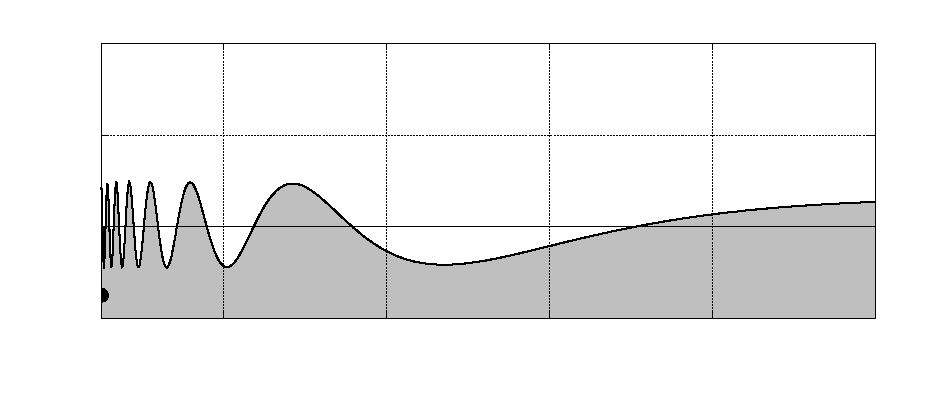
\includegraphics{./Analytic004}}%
    \gplfronttext
  \end{picture}%
\endgroup

  \caption{$t=3$ s.}
 \end{subfigure} \\
  \begin{subfigure}{\textwidth}
  % GNUPLOT: LaTeX picture with Postscript
\begingroup
  \makeatletter
  \providecommand\color[2][]{%
    \GenericError{(gnuplot) \space\space\space\@spaces}{%
      Package color not loaded in conjunction with
      terminal option `colourtext'%
    }{See the gnuplot documentation for explanation.%
    }{Either use 'blacktext' in gnuplot or load the package
      color.sty in LaTeX.}%
    \renewcommand\color[2][]{}%
  }%
  \providecommand\includegraphics[2][]{%
    \GenericError{(gnuplot) \space\space\space\@spaces}{%
      Package graphicx or graphics not loaded%
    }{See the gnuplot documentation for explanation.%
    }{The gnuplot epslatex terminal needs graphicx.sty or graphics.sty.}%
    \renewcommand\includegraphics[2][]{}%
  }%
  \providecommand\rotatebox[2]{#2}%
  \@ifundefined{ifGPcolor}{%
    \newif\ifGPcolor
    \GPcolortrue
  }{}%
  \@ifundefined{ifGPblacktext}{%
    \newif\ifGPblacktext
    \GPblacktexttrue
  }{}%
  % define a \g@addto@macro without @ in the name:
  \let\gplgaddtomacro\g@addto@macro
  % define empty templates for all commands taking text:
  \gdef\gplbacktext{}%
  \gdef\gplfronttext{}%
  \makeatother
  \ifGPblacktext
    % no textcolor at all
    \def\colorrgb#1{}%
    \def\colorgray#1{}%
  \else
    % gray or color?
    \ifGPcolor
      \def\colorrgb#1{\color[rgb]{#1}}%
      \def\colorgray#1{\color[gray]{#1}}%
      \expandafter\def\csname LTw\endcsname{\color{white}}%
      \expandafter\def\csname LTb\endcsname{\color{black}}%
      \expandafter\def\csname LTa\endcsname{\color{black}}%
      \expandafter\def\csname LT0\endcsname{\color[rgb]{1,0,0}}%
      \expandafter\def\csname LT1\endcsname{\color[rgb]{0,1,0}}%
      \expandafter\def\csname LT2\endcsname{\color[rgb]{0,0,1}}%
      \expandafter\def\csname LT3\endcsname{\color[rgb]{1,0,1}}%
      \expandafter\def\csname LT4\endcsname{\color[rgb]{0,1,1}}%
      \expandafter\def\csname LT5\endcsname{\color[rgb]{1,1,0}}%
      \expandafter\def\csname LT6\endcsname{\color[rgb]{0,0,0}}%
      \expandafter\def\csname LT7\endcsname{\color[rgb]{1,0.3,0}}%
      \expandafter\def\csname LT8\endcsname{\color[rgb]{0.5,0.5,0.5}}%
    \else
      % gray
      \def\colorrgb#1{\color{black}}%
      \def\colorgray#1{\color[gray]{#1}}%
      \expandafter\def\csname LTw\endcsname{\color{white}}%
      \expandafter\def\csname LTb\endcsname{\color{black}}%
      \expandafter\def\csname LTa\endcsname{\color{black}}%
      \expandafter\def\csname LT0\endcsname{\color{black}}%
      \expandafter\def\csname LT1\endcsname{\color{black}}%
      \expandafter\def\csname LT2\endcsname{\color{black}}%
      \expandafter\def\csname LT3\endcsname{\color{black}}%
      \expandafter\def\csname LT4\endcsname{\color{black}}%
      \expandafter\def\csname LT5\endcsname{\color{black}}%
      \expandafter\def\csname LT6\endcsname{\color{black}}%
      \expandafter\def\csname LT7\endcsname{\color{black}}%
      \expandafter\def\csname LT8\endcsname{\color{black}}%
    \fi
  \fi
    \setlength{\unitlength}{0.0500bp}%
    \ifx\gptboxheight\undefined%
      \newlength{\gptboxheight}%
      \newlength{\gptboxwidth}%
      \newsavebox{\gptboxtext}%
    \fi%
    \setlength{\fboxrule}{0.5pt}%
    \setlength{\fboxsep}{1pt}%
\begin{picture}(8640.00,3600.00)%
    \gplgaddtomacro\gplbacktext{%
    }%
    \gplgaddtomacro\gplfronttext{%
      \csname LTb\endcsname%
      \put(176,2019){\makebox(0,0){\strut{}$\eta$}}%
      \put(4528,154){\makebox(0,0){\strut{}$r$}}%
      \csname LTb\endcsname%
      \put(682,704){\makebox(0,0)[r]{\strut{}$-4$}}%
      \csname LTb\endcsname%
      \put(682,1581){\makebox(0,0)[r]{\strut{}$0$}}%
      \csname LTb\endcsname%
      \put(682,2458){\makebox(0,0)[r]{\strut{}$4$}}%
      \csname LTb\endcsname%
      \put(682,3335){\makebox(0,0)[r]{\strut{}$8$}}%
      \csname LTb\endcsname%
      \put(1987,484){\makebox(0,0){\strut{}$0.2$}}%
      \csname LTb\endcsname%
      \put(3551,484){\makebox(0,0){\strut{}$0.4$}}%
      \csname LTb\endcsname%
      \put(5115,484){\makebox(0,0){\strut{}$0.6$}}%
      \csname LTb\endcsname%
      \put(6679,484){\makebox(0,0){\strut{}$0.8$}}%
      \csname LTb\endcsname%
      \put(8243,484){\makebox(0,0){\strut{}$1$}}%
    }%
    \gplbacktext
    \put(0,0){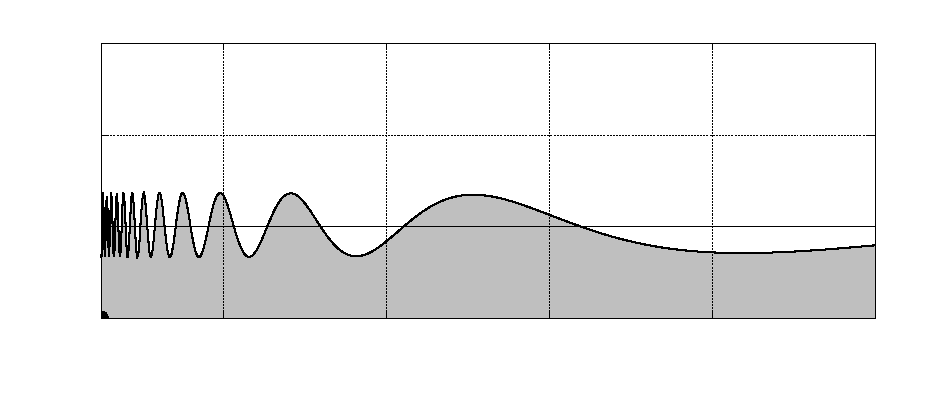
\includegraphics{./Analytic005}}%
    \gplfronttext
  \end{picture}%
\endgroup

  \caption{$t=4$ s.}
 \end{subfigure}
 \end{centering}
\end{figure}




\end{document}
